\section{イントロダクション}
\subsection{極端降雨気象}
日本において地上気象観測は古くから行われており、近年では全国配備された自動気象
データ収集システム(AMeDAS)や、C バンドレーダー・X バンドレーダーによって、気
温・気圧などの気象パラメータと降水分布がほぼリアルタイムに観測されるような態勢が
確立されている。しかしながら、このような最先端の気象観測網をもってしても、ゲリラ豪
雨や線状降水帯、さらには台風に伴う豪雨など、大規模災害に直結し、かつ近年多発傾向に
ある極端気象の予測は、依然として困難である。
気象庁のホームページ\url{https://www.jma.go.jp/jma/kishou/know/yougo_hp/kousui.html}
では降雨の内、「著しい災害が発生した顕著な大雨現象」と豪雨としている。一方、集中豪
雨を「同じような場所で数時間にわたり強く降り、100mm から数百 mm の雨量をもたらす
雨」と説明している。これらのような極端降雨現象は、最先端の技術でも予測が大変難しい
ことが知られている。集中豪雨の中でも、稀にしか発生しないような大雨は、極端豪雨、極
端降雨気象などと呼ばれる。
近年における降雨状況を、 Masaki [2020]の発表をもとにまとめる。気象庁における統計
データ [1]では、アメダスによる 1 時間降水量が 50、80、200、400mm以上の降雨の年間発
生件数の、1975 年以降の変化傾向はいずれにおいても増加トレンドにあることが示されて
いる。(図1)

\begin{figure}[H]
	\begin{tabular}{cc}
		\begin{minipage}[t]{1.0\hsize}
		\begin{center}
		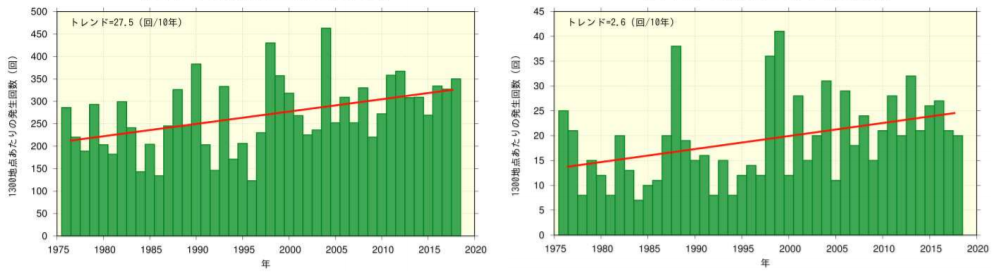
\includegraphics[width=1.0\linewidth,clip]{fig/intro/kisyotyo-repo-chart50-80.png}
		\subcaption{50mm(左)、80mm(右)}
		\label{a}
		\end{center}
		\end{minipage}\\
		
		\begin{minipage}[t]{1.0\hsize}	
		\begin{center}
		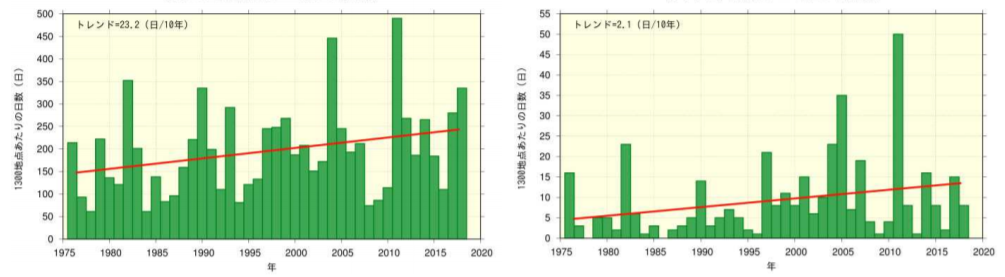
\includegraphics[width=1.0\linewidth,clip]{fig/intro/kisyotyo-repo-chart200-400.png}
		\subcaption{200mm(左)、400mm(右)}
		\label{b}
		\end{center}
		\end{minipage}
	\end{tabular}
	\caption{1976-2018年期間の全国のアメダスの1時間降水量50mm、80mm (a)、200mm、400mm (b) 以上の年間発生回数の変化。棒グラフは全国のアメダスによる観測値を 1300 地点当たりに換算した値、直線は長期変化傾向を表す。}
\end{figure}
